% Preamble (Angaben gelten für das ganze Dokument)
% Hilfe für Bibtex Einträge: https://www.literatur-generator.de
% ------------------------------------------------
% rote Umrandungen bei Verlinkungen entfernen: hidelinks
% 12pt als Standardschriftgröße
% A4-Dokument
% twoside (zweiseitiges Dokument): nur so werden verschiedene Fußzeilen für gerade bzw. ungerade Seitenzahlen übernommen
% article: Dokumentvorlage
\documentclass[hidelinks,12pt,a4paper,twoside]{article}
% Einbinden von Paketen
% ---------------------
\usepackage{titlesec} 						% ermöglicht die Verwendung der title- und section-Befehle
\usepackage[utf8]{inputenc}					% ermöglicht das Verwenden von Umlauten - linux od osx
\usepackage{makecell}
\usepackage[top=3.5cm,left=3cm,right=2cm,bottom=2.5cm,headsep=0.3in,headheight=1in]{geometry} % Seitenränder
\usepackage{graphicx} 						% ermöglicht die Verwendung des includegraphics-Befehls zur Einbindung von Bildern
\usepackage{fancyhdr} 						% ermöglicht die einfache Erstellung von Kopf- und Fußzeilen
\usepackage{setspace} 						% ermöglicht Veränderung verschiedener Abstände
\usepackage{array} 							% ermöglicht unter anderem das Erstellen von benutzerdefinierten Vorlagen für Tabellenspalten
\usepackage[export]{adjustbox} 				% Umrandung von Bildern
\usepackage[nottoc,numbib]{tocbibind} 		% ermöglicht die Erstellung eines Inhaltsverzeichnisses
\usepackage{tocloft}
\setlength{\cftsubsecnumwidth}{3em} 		% Set distance between number and text of subsection in table of contents
\usepackage{color} 							% ermöglicht das Erstellen von benutzerdefinierten Farben

\usepackage{longtable}						% Unterstützung für mehrseitige Tabellen
\usepackage[ngerman]{babel}					% Deutsche Bezeichnungen 

\usepackage[backend=biber,citestyle=verbose, bibstyle=verbose]{biblatex} %mehrsprachiges Bibliotheks(Literatur-)verzeichnis
\usepackage[babel,german=guillemets]{csquotes} %deutsches Anführungszeichen
\addbibresource{bibliography.bib}

\usepackage{blindtext} 						% Blindtext
\usepackage{url} 							% Formatierung von URLs
\usepackage[bottom,hang,stable]{footmisc} 	% Fußnoten immer am unteren Ende der Seite
\usepackage{caption} 						% ermöglicht das Anpassen von diversen Beschriftungen
\usepackage{subcaption} 					% ermöglicht das Erstellen von Unterbezeichnungen (subfigures)
\usepackage{hyperref} 						% Hyperlinks im Dokument
\usepackage{pdfpages} 						% einbinden von PDF-Dateien
\usepackage{amsmath} 						% grundlegende mathematische Funktionen

\usepackage{listings,chngcntr} 				% kapitelweise Nummerierung für Codeabschnitte
\usepackage{listings,xcolor} 				% ermöglicht das Einbinden von Codesegmenten
\usepackage{listingsutf8} 					% ermöglicht das Einbinden von Codesegmenten

\usepackage{float} 							% Positionierung verschiedener Objekte
\usepackage{footnote} 						% ermöglicht das Anpassen von Fußnoten
\usepackage{enumitem} 						% ermöglicht das Anpassen von Aufzählungen
\usepackage{longtable} 						% erlaubt mehrseitige Tabellen
\usepackage{url} 							% gibt eine schöner formatierte Internetadresse aus


% allgemein gültige Formateinstellungen
% -------------------------------------
\renewcommand{\familydefault}{\sfdefault} 	% set Font-Family to a similar font like Arial
\raggedbottom 								% Abschnitte werden nicht auseinander gezogen, um den restlichen Platz auf einer Seite zu füllen
%\raggedright 								% gesamtes Dokument linksbündig (auch Paragraphen) OHNE Silbentrennung

\usepackage{ragged2e}						% gesamtes Dokument linksbündig (auch Paragraphen) MIT Silbentrennung
\RaggedRight

\onehalfspacing 							% 1.5-facher Abstand zwischen den Zeilen

\renewcommand{\arraystretch}{1.2} 			% Vergrößerung des Abstands zwischen den Tabellenzeilen
\newcolumntype{C}[1]{>{\centering\arraybackslash}p{#1}} % erstellen eines Spaltentyps mit zentriertem Inhalt unter der Angabe einer Spaltenbreite
\newcolumntype{L}[1]{>{\raggedright\arraybackslash}p{#1}} % erstellen eines Spaltentyps mit linksbündigem Inhalt unter der Angabe einer Spaltenbreite

\setlength{\footnotemargin}{0.5cm} 			% Abstand zwischen Fußnotennummer und -text
\setlist{nosep} 							% zusätzliche Abstände bei Aufzählungen entfernen
\setlength{\parskip}{1em} 					% Abstand nach einem Absatz

% Abstände vor und nach Überschriften auf den verschiedenen Ebenen
\titlespacing\section       {0pt}{0pt plus 0pt minus 2pt}{0pt plus 2pt minus 2pt}
\titlespacing\subsection    {0pt}{0pt plus 0pt minus 2pt}{0pt plus 2pt minus 2pt}
\titlespacing\subsubsection {0pt}{0pt plus 0pt minus 2pt}{0pt plus 2pt minus 2pt}

% Formateinstellungen für Codesegmente
% ------------------------------------
\usepackage{caption}
\usepackage{minted} 						% für schöne Darstellung von Code
\usepackage{dingbat}						% für Sonderzeichen wie \carriagereturn

\setminted{
	autogobble,								% rückt Code soweit nach links wie möglich
	stepnumber=2,							% nur jede gerade Zeilennummer wird angezeigt
	fontfamily=tt,
	linenos=true,
	numberblanklines=true,
	numbersep=5pt,
	gobble=0,
	frame=single,
	framerule=0.4pt,
	framesep=2mm,
	funcnamehighlighting=true,
	tabsize=4,
	obeytabs=false,
	breaklines,
	breakafter=">/,
	breakbefore=. ,
	breaksymbolindentright=10pt,
	breaksymbolsepright=0pt
}

\newmintedfile[csharpcode]{csharp}{}
\newmintedfile[xamlcode]{xml}{}
\newmintedfile[bashcode]{bash}{}

\usepackage{etoolbox}
\AtBeginEnvironment{longlisting}{\dontdofcolorbox}
\def\dontdofcolorbox{\renewcommand\fcolorbox[4][]{##4}}		% zum Unterbinden des roten Rahmens im Quellcode um ein $-Zeichen

\newenvironment{longlisting}{\captionsetup{type=listing} \linespread{1.1}}{} % 1.1 facher Zeilenabstand bei listings

% Anlegen von benutzerdefinierten Farben für das Hervorheben bestimmter Teile des Codes
\definecolor{shblue}{rgb}{0.13,0.13,1} % Farbe für Schlüsselwörter
\definecolor{shgreen}{rgb}{0,0.5,0} % Farbe von Kommentaren
\definecolor{shred}{rgb}{0.9,0,0} % Farbe von Zeichenfolgen
\definecolor{lightgray}{gray}{0.95} % Hintergrundfarbe
\definecolor{maroon}{rgb}{0.5,0,0}
\definecolor{bg}{rgb}{0.95,0.99,0.99}

% benutzerdefiniertes Syntax-Highlighting für XAML
\lstdefinelanguage{XAML}
{
	morestring=[s]{"}{"},
	moredelim=[s][\color{black}]{>}{<},
	moredelim=[s][\color{maroon}]{<}{\ },
	moredelim=[s][\color{maroon}]{</}{>},
	moredelim=[l][\color{maroon}]{/>},
	moredelim=[l][\color{maroon}]{>},
	morecomment=[s]{<?}{?>},
	morecomment=[s]{<!--}{-->},
	commentstyle=\color{shgreen},
	stringstyle=\color{shblue},
	identifierstyle=\color{shred}
}

% spezifische Einstellungen für verschiedene Sprachen
\lstdefinestyle{csharp}
{
	language=[Sharp]C,
	commentstyle=\color{shgreen}, % Farbe für Kommentare
	keywordstyle=\color{shblue},
	stringstyle=\color{shred}
}

\lstdefinestyle{xaml}
{
	language=XAML
}

\skip\footins 30pt				% etwas größerer Abstand oberhalb Fußnote

% Anpassung diverser Beschriftungen
\captionsetup[listing] {labelfont=bf,textfont=it,format=hang,justification=raggedright}
\captionsetup[table]   {labelfont=bf,textfont=it,format=hang,justification=raggedright}
\captionsetup[figure]  {labelfont=bf,textfont=it,format=hang,justification=raggedright}

\captionsetup[figure]  {name=Abbildung} 		% Abbildungen
\captionsetup[table]   {name=Tabelle} 			% Tabellen
\captionsetup[longlisting]{name=Codeabschnitt}	% Codeabschnitte -> fkt. leider nicht


% kapitelweise Nummerierung
\numberwithin{figure}{section}				% kapitelweise Nummerierung für Grafiken
\numberwithin{table}{section}				% kapitelweise Nummerierung für Tabellen
\numberwithin{listing}{section}				% kapitelweise Nummerierung für Codeabschnitte

\usepackage{tcolorbox}
\newtcolorbox[blend into=figures]{myfigure}[2][]{float=htb,capture=hbox,
	blend before title code={\fbox{##1}\ },title={#2},every float=\centering,#1}



% Quellennachweise in weiterer Datei anlegen
\bibliography{bibliography}
\newcommand{\diplomatitle}{MazeRun}

\newcommand{\supervisor}{Dipl.-Ing. Rusch Helmut Elmar}

\newcommand{\emplA}{Semih Can}
\newcommand{\emplLastA}{BURCAK}
\newcommand{\emplAbbrA}{SCB}

\newcommand{\emplB}{Semih}
\newcommand{\emplLastB}{SÖNMEZ}
\newcommand{\emplAbbrB}{SS}

\newcommand{\emplC}{Manuel}
\newcommand{\emplLastC}{RATH}
\newcommand{\emplAbbrC}{MR}

\newcommand{\emplD}{Mateo}
\newcommand{\emplLastD}{HERCEG}
\newcommand{\emplAbbrD}{MH}

\newcommand\SecAuth[1]{\def\@SecAuth{#1}}

\newcommand{\DADate}{2022\textbar20}

\newcommand{\PrintDate}{08.04.2022}

\pagestyle{fancy}
% Kopf- und Fußzeile
% ------------------
% Kopfzeile: links: Logo HTL Rankweil; mitte: Schulbezeichnung; rechts: Logo HTL
\lhead{\hspace{0.2cm} 
\includegraphics[height=1.04cm]{img/htlr_logo.png}}
\chead{\textbf{HTBLuVA  Rankweil} 
	\\[0.05in]
	\footnotesize{\textit{Höhere Lehranstalt für Elektronik und Technische Informatik}}}
\rhead{
\includegraphics[height=1.04cm]{img/htl_logo.jpg} \hspace{0.2cm}}

% Fußzeile
\fancyfoot{} 


\begin{document}
	% Titelseite
	\begin{center}
		\textbf {\huge {\uppercase {MazeRun}}}
		\par \large {Gesamtprojekt}
		\par \textbf {\huge {\uppercase {Thema}}}
		\vspace{0.3cm}
		\linebreak
		
\includegraphics[frame, height=6cm]{img/title_placeholder.png}
	\end{center}
	
	\vfill % damit der folgende am Blattende positioniert wird
	

\begin{minipage}[t] {0.4\textwidth}
	\textbf{Teammitglieder:} \\
	\emplLastA \\
	\emplLastB \\
	\emplLastC \\
	\emplLastD \\
\end{minipage}
\begin{minipage}[t] {0.4\textwidth}
	\textbf{Betreuer:} \\		
	\supervisor \\
\end{minipage}

	\par Rankweil, am \PrintDate \\		

	\noindent\rule{\textwidth}{0.4pt}
	Abgabevermerk:
	\linebreak

	\begin{tabular}{p{7cm}C{6cm}}
		\hspace{1cm} DA original, am \PrintDate & ........................................ \\ 
		& \supervisor \vspace{0.5cm} \\
		
	\hspace{1cm} DA digital, am \PrintDate & ........................................ \\ 
		& \supervisor \\
	\end{tabular}
	
	% Leere Seite
	\pagebreak
	\thispagestyle{empty}
	\cleardoublepage
	\pagebreak
	
	% ab jetzt andere Fußzeile
	%\fancyhead{}
	%\renewcommand{\headrulewidth}{0.0pt}
	\SecAuth{\emplLastA, \emplLastB, \emplLastC, \emplLastD} % festlegen der Verfasser dieses Kapitels
	
	\pagenumbering{Roman}
	\fancyfoot[LE,RO]{\thepage}
	\fancyfoot[LO,RE]{\DADate~\textbar~\diplomatitle~\textbar ~\@SecAuth}
	\renewcommand{\footrulewidth}{0.4pt} % anzeigen Separator-Strich in der Fußzeile (standardmäßig deaktiviert)
	
	
% Eidesstattliche Erklärung (Deutsch)
\section*{Eidesstattliche Erklärung}
Ich erkläre an Eides statt, dass ich die vorliegende Diplomarbeit selbständig und ohne fremde
Hilfe verfasst, andere als die angegebenen Quellen und Hilfsmittel nicht benutzt und die den
benutzten Quellen wörtlich und inhaltlich entnommenen Stellen als solche erkenntlich
gemacht habe.

\vspace{0.3cm}
\par Rankweil, am \PrintDate
\linebreak
\linebreak
\begin{tabular}{p{7cm}C{5cm}}
	& ........................................ \\[-1em]
	& \emplA \\ [1.5em]
	& ........................................ \\[-1em]
	& \emplB \\ [1.5em]
	& ........................................ \\[-1em]
	& \emplC \\ [1.5em]
	& ........................................ \\[-1em]
	& \emplD \\ [1.5em]
\end{tabular}

 % 
\pagebreak

% Abkürzungen und Hinweise
\section*{Abkürzungen \& Hinweise}
\begin{singlespace}	
	\begin{tabular}{ll}
		DA     & Diplomarbeit \\
		WPF    & Windows Presentation Foundation \\
		CAD    & Computer-aided design \\
		Regex  & Regular expression \\
		GPL    & General Public License  \\
		SI     & Internationales Einheitensystem \\
		COM    & Component Object Model \\
		GUI    & Graphical User Interface \\
	\end{tabular}
\end{singlespace}

\pagebreak
	
% Inhaltsverzeichnis
% ------------------
\singlespacing % Zeilenabstand verringern

% Inhaltsverzeichnis in Inhaltsverzeichnis 
% s. auch https://www.latex-tutorial.com/tutorials/table-of-contents/
%\renewcommand{\tableofcontents}{\begingroup
%	\tocfile{Inhaltsverzeichnis}{toc}
%	\endgroup}

\tableofcontents % eigentlicher Befehl für das Anlegen des Inhaltsverzeichnisses
\onehalfspacing % standardmäßigen Zeilenabstand wiederherstellen
\pagebreak

% ab jetzt mit arabischen Seitennummern
\renewcommand{\thepage}{\arabic{page}}% Arabic page numbers

% eigentlicher Inhalt des Dokuments
% --------------------
\SecAuth{\emplLastA} % festlegen der Verfasser dieses Kapitels

% DA Dokumentation (Deutsch)
\addcontentsline{toc}{section}{DIPLOMARBEIT DOKUMENTATION}
\section *{DIPLOMARBEIT DOKUMENTATION}
	\SecAuth{\emplLastA} % festlegen der Verfasser dieses Kapitels für die Fußzeile

\begin{tabular}{@{}p{5cm}p{8cm}}
Name der Verfasser~\textbar~innen & \emplA, \emplB, \emplC, \emplD \\

Jahrgang ~\textbar~ Schuljahr & 5Klasse ~\textbar~ 20SJ~\textbar~20SJ \\

THEMA der Diplomarbeit & Spiel- und Kontrollerentwicklung \\

Aufgabenstellung & Es ist ein Videospiel welches mit einem Kontroller einfach zu bedienen ist. Dabei soll auch eine kleine Geschichte mit dem Spiel erzählt werden. Die Diplomarbeit soll auch ein How-To für Erstellung eines Unity-Spiels gesteuert durch Megacard und ESP Kontrollers sein.  \\
\end{tabular}

\pagebreak

\subsection *{Individuelle Themenstellung im Rahmen des Gesamtprojektes}
\begin{tabular}{@{}p{5cm}p{8cm}}

	\emplA & 	Herr Burcak macht das Projektmanagement des Projektes, die Auslesung der Kontroller Signale und das Audio, Story, Benutzeroberfläche, Webserver und den Multiplayer-Teil des Spiels.  \\
		
	\emplB & 	Die grundlegenden Bewegungen vom Charakter und Gegner, sowie die Physik des Spiels werden von Semih Sönmez programmiert. Auch die Umgebung mit Missionen und Levels wird vom Herrn Sönmez entwickelt.  \\
		
	\emplC & 	 
	
	Manuel Rath ist für die Steuerung des Spiels zuständig. Der Kontroller wird aus der Megacard von der Schule erstellt. Die Kommunikation zwischen Kontroller und Spiel erfolgt über USB oder Bluetooth.  \\

	\emplD & 	Herr Herceg entwickelt den 2. Kontroller für die Steuerung. Die Daten werden mittels ESP Moduls per WLAN oder Bluetooth an den PC gesendet. Zudem werden für beide Kontroller ein Gehäuse und Stromversorgung angelegt.  \\

Realisierung & Bei Realisierung angeben, sonst freilassen.  \\

Ergebnisse & Das Spiel ist in Unity-3D zu realisieren. Die Highscores werden auf einem zentralen Server gespeichert. Die Eingaben vom Kontroller sollen von der Megacard/ESP ausgelesen und mittels USB/WLAN/Bluetooth an das Spiel weitergeitet werden und die Spielfigur soll sich entsprechend bewegen. Der aus einem eigenen Akku und Gehäuse bestehender Kontroller soll auch als Feedback beim Spielen vibrieren.   \\

Einsichtnahmen**) & Archiv der HTL Rankweil, \newline www.diplomarbeiten.berufsbildendeschulen.at \\
\end{tabular}
 % 
\pagebreak

% DA Dokumentation (Englisch)
\addcontentsline{toc}{section}{DIPLOMA THESIS DOCUMENTATION}
\section *{DIPLOMA THESIS DOCUMENTATION}

\begin{tabular}{@{}p{5cm}p{8cm}}
Author(s) & \emplA, \emplB, \emplC, \emplD \\

Form ~\textbar~ Academic year & 5Klasse ~\textbar~ 21SJ~\textbar~22SJ \\

Diploma Thesis Topic & Game and Controllerdevelopment \\

Assignment of Tasks & At the end of this diploma thesis a multiplayer game and two controllers made with the inhouse Megacard and ESP to control the game will be developed. \\
\end{tabular}

\pagebreak

\subsection *{Individual Tasks within the overall project}
\begin{tabular}{@{}p{5cm}p{8cm}}

	\emplA & 	Mr. Burcak will do the management of this project, reading and evaluating signals from the controllers, the audio, the story, UI, Webserver and the multiplayer of the game.\\
		
	\emplB & 	 The character movements and the physics of the game will be developed by Mr. Sönmez. The environment, missions and levels will also be developed by Mr. Sönmez. \\
		
	\emplC & 	Mr. Rath is responsible for the controls of the game. The Megacard-Controller will be developed by him and it will communicate via USB and Bluetooth. \\

	\emplD & 	 Mr. Herceg is also responsible for the controls of the game. He will develop the second controller, it will be developed with ESP and it will communicate via WIFI and Bluetooth.\\

Realisation & Bei Realisierung angeben, sonst freilassen.  \\

Result & The game is to be developed in Unity-3D. The highschores will be saved on a central server. The inputs from the controllers are to be sent via USB/WIFI/Bluetooth to the game and character should move according to the input. The controllers will vibrate as feedback and have their own power source. \\

Publication**) & Archiv der HTL Rankweil, \newline  www.diplomarbeiten.berufsbildendeschulen.at \\
\end{tabular}
 % 
\pagebreak

% zusammenfassung
\addcontentsline{toc}{section}{ZUSAMMENFASSUNG}
\section*{ZUSAMMENFASSUNG}
Darlegung des Themas, der Fragestellung, der Problemformulierung sowie der Ergebnisse.
Kurze, prägnante Information über den Inhalt der Arbeit; keine Wertungen oder Meinungen (allerdings in ganzen Sätzen!).

\subsection*{A Aufgabenstellung}
\begin{itemize}
	\item Von welchem Wissens- oder Entwicklungsstand im Umfeld der Aufgabenstellung wird ausgegangen bzw. welche Ergebnisse und Erkenntnisse gibt es bereits zum Thema?
	\item Welches Ziel soll erreicht werden?
	\item Warum und für wen ist das definierte Ziel von Interesse?
\end{itemize}

\subsection*{B Umsetzung}
\begin{itemize}
	\item Auf welche fachtheoretischen/-praktischen Grundlagen wurde zurückgegriffen?
	\item Welche Lösungsansätze/Methoden wurden gewählt?
	\item Warum gerade diese und keine anderen?
	\item Welche Alternativen gäbe es noch?
	\item Es könnte ev. auf den Bearbeitungsprozess im Team eingegangen werden (Reflexion).
\end{itemize}

\subsection*{C Ergebnisse}
\begin{itemize}
	\item Worin besteht der Beitrag zur Lösung der Aufgabenstellung? (Website-Erstellung, Marketingkonzept, …)
	\item Welches Produkt soll erstellt werden?
	\item Es könnte ev. darauf eingegangen werden, ob die Diplomarbeit bei Wettbewerben eingereicht wurde oder ob es Prämierungen gab.
\end{itemize}


Das sind Fragestellungen, die in der ZUSAMMENFASSUNG und auch in der Übersetzung in englischer Sprache im ABSTRACT vorkommen können (als Vorschlag – je nach Projekt ergeben sich auch andere Fragen).
Die Struktur mit A Aufgabenstellung, B Umsetzung und C Ergebnisse muss aber jedenfalls eingehalten werden!
 % 
\pagebreak

% Abstract (English)
\addcontentsline{toc}{section}{Abstract (English)}
\section *{Abstract (English)}
s. Zusammenfassung % English
\pagebreak
	
% Kapitel 1: Pflichtenheft
% -------------


\emph{\textbf{Diplomarbeit "MazeRun" 5AHEL 2021-22}}

\hypertarget{lastenheft--pflichtenheft}{%
\section{Lastenheft / Pflichtenheft}\label{lastenheft--pflichtenheft}}

\hypertarget{kurzbeschreibung}{%
\subsection{Kurzbeschreibung}\label{kurzbeschreibung}}
\begin{quote}
	Das Spiel ist in der 3D-Umgebung in Unity zu realisieren. Die Highscores
	werden auf einem zentralen Server gespeichert. Die Eingaben vom
	Kontroller sollen von der Megacard/ESP ausgelesen und mittels USB/WLAN
	evtl. Bluetooth an das Spiel weitergeitet werden. Anschließend sollte
	sich die Spielfigur entsprechend bewegen. Der aus einem eigenen Akku und
	Gehäuse bestehender Kontroller soll auch als Feedback beim Spielen
	vibrieren. Die Diplomarbeit soll auch ein How-To für Erstellung eines
	Unity-Spiels/Megacard \& ESP Kontrollers sein.
\end{quote}


\hypertarget{aufgaben-einzelner-projektmitglieder}{%
\subsection{Aufgaben einzelner
Projektmitglieder}\label{aufgaben-einzelner-projektmitglieder}}

\begin{longtable}{l l}

\textbf{Name} & \textbf{Individuelle Themenstellung}\tabularnewline

\endhead
Semih Can Burcak (Hauptverantwortlich) & \makecell[tl]{Projektmanagement /
	Spielsoftwareentwicklung \\ / Spieldesign / Onlinespielentwicklung  } \\
Semih Sönmez & \makecell[tl]{Spielsoftwareentwicklung / Spieldesign} \\
Manuel Rath & \makecell[tl]{Schaltungsdesign / Analoglayout \\/ Microcontroller
Programmierung} \\
Mateo Herceg & \makecell[tl]{Schaltungsdesign / Analoglayout \\/ Microcontroller
Programmierung} \\

\end{longtable}

\hypertarget{projektziele-nach-smart}{%
\subsection{Projektziele nach SMART}\label{projektziele-nach-smart}}
\begin{quote}

\hypertarget{spezifisch}{%
\subsubsection{Spezifisch}\label{spezifisch}}

Das Spiel soll professionell aussehen und ohne Probleme online von jeden
gespielt werden können. Die Spielstände der Spieler sollen einwandfrei
auf einem Server gespeichert werden. Die selbstgemachten Kontroller
sollen ebenfalls einwandfrei funktionieren. Die Verbindung zwischen dem
Spiel (C\#) und Kontroller (C) soll automatisch sein bzw. die Kontroller
sollen Plug \& Play Kontroller sein.

\hypertarget{messbar}{
\subsubsection{Messbar}\label{messbar}}

Jede neue Funktion des Spiels soll ausführlich getestet werden. Die
Verbindung des Kontrollers zum Spiel wird im Spiel getestet, indem wir
schauen ob die Tasten und die Joysticks das machen, was wir wollen.

Nachdem das Spiel und die Kontroller fertig entwickelt wurden, wird
alles nochmals getestet um evtl. Bugs zu finden und zu schauen ob alles
wie geplant funktioniert.

\subsubsection{Realistisch}\label{realistisch}

Die Programmiersprachen C\# und C wurden im Unterricht schon
durchgenommen. Die Kommunikation zwischen PC und µC wurde noch nicht
gemacht, aber mit der richtigen Hilfe bzw. Professor sollte es
realisierbar sein. Das Projekt wird Schritt für Schritt entwickelt und
ist daher realistisch.

\hypertarget{terminiert}{%
\subsubsection{Terminiert}\label{terminiert}}


\begin{longtable}[]{@{}ll@{}}

\emph{Datum} & \emph{Meilenstein}\tabularnewline

\endhead

\textbf{Anfang Oktober (04.10.2021)} & Auswahl und Layout der Hardware,
Anfangen das Spiel zu programmieren\tabularnewline
\textbf{Anfang November (01.11.2021)} & Die Umgebung/Charaktere des
Spiels sollen fertig sein,\tabularnewline
\textbf{Mitte bis Ende November (30.11.2013)} & Entwicklungsphase des
Spiels fertig,\tabularnewline
\textbf{Dezember und Jänner} & Online-Funktion des Spiels
programmieren\tabularnewline
\textbf{Ende 1. Halbjahr (14.02.2022)} & Fertigstellung des
Projekts\tabularnewline

\caption{Meilensteine}

\end{longtable}

Das Projekt soll in diesem Halbjahr (Wintersemester SJ 2021-22)
fertiggestellt werden.

\end{quote}

\hypertarget{produkteinsatz}{%
\subsection{Produkteinsatz}\label{produkteinsatz}}
\begin{quote}
Das Spiel sollte mit einem Computer gestartet werden, der Zugang auf ein
Internet verfügt. Die Kontroller sollten entweder über USB, Bluetooth
oder WLAN mit dem PC verbunden sein. Bei kabellosem Kontroller soll
sicher gestellt werden, dass die Batterie noch Energie hat.
\end{quote}
\hypertarget{funktionale-anforderungen}{%
\subsection{Funktionale Anforderungen}\label{funktionale-anforderungen}}
\begin{quote}
Durch den Kontroller sollten folgende Bewegungen durchgeführt werden
können:

\begin{itemize}
\item
  Grundlegende Bewegungen (vorne, hinten, rechts, links,)
\item
  Springen des Spielers
\item
  Bewegung der Kamera
\end{itemize}
\end{quote}
\hypertarget{projektphasen-und-meilensteine}{%
\subsection{Projektphasen und
Meilensteine}\label{projektphasen-und-meilensteine}}
 
\hypertarget{spiel}{%
\subsubsection{Spiel}\label{spiel}}
\begin{quote}
Zuerst sollen die Grundlegenden Bewegungen vom Charakter programmiert
werden. Anschließend kann das Multiplayer Spielmodus programmiert
werden. Das Know-How soll bis das Spiel bereit ist (Bewegungen, Umgebung
etc.), um es online zu spielen, erschafft werden.
\end{quote}
\hypertarget{kontroller}{%
\subsubsection{Kontroller}\label{kontroller}}
\begin{quote}
Zuerst werden Layout und Schaltplan erstellt und daraus wird die
Leiterplatte entstehen. In der zwischen Zeit werden die einzelnen
Bauteile bestellt und Angesteuert. Nach der Fertigung der Hardware
starten wir mit einzelnen Testprogrammen, die wir später für die fertige
Software brauchen. Zu guter Letzt wird ein passendes Gehäuse mit einem
Akku konstruiert.
\end{quote}
\hypertarget{arbeitspakete-aufgelistet}{%
\subsection{Arbeitspakete
(aufgelistet)}\label{arbeitspakete-aufgelistet}}

\hypertarget{semih-can-burcak}{%
\subsubsection{Semih Can Burcak}\label{semih-can-burcak}}

\begin{itemize}
\item
  Benutzeroberfläche des Spiels

  \begin{itemize}
  \item
    Username Eingabe - must have
  \item
    Wahlmenü (Einzelspieler oder Mehrspieler, Level usw.) - must have
  \item
    Es soll aus HTL Rankweil Farben bestehen (Blau, Grau, Schwarz)
  \item
    Benutzerfreundlich gestalten - must have
  \end{itemize}
\item
  Audio

  \begin{itemize}
  \item
    Copyrightfreie Audios verwenden - must have 
  \item
    Die Musik und die Sounds sollen dem Spiel mehr energetisch machen -
    must have
  \item
    Lautstärke gut einstellen (nicht zu laut oder leise)
  \end{itemize}
\item
  Multiplayer - must have

  \begin{itemize}
  \item
    Webserver einrichten 
  \item
    Datenbank erstellen
  \item
    Datenbank und Webserver mit Unity verbinden
  \item
    Schauen, dass jeder Spieler ein Charakter zugeteilt kriegt
  \end{itemize}
\item
  Story

  \begin{itemize}
  \item
    Es soll nicht langweilig sein und Interesse wecken - must have
  \item
    Zuerst auf dem Papier das Konzept bzw. Story festigen und erst
    programmieren
  \end{itemize}
\item
  Projektmanagement - must have

  \begin{itemize}
  \item
    Das Team soll immer organisiert bleiben
  \item
    Jeder soll seine Aufgaben rechtzeitig erledigen, damit kein
    Zeitdruck entsteht
  \item
    Ordentlich Dokumentieren
  \end{itemize}
\end{itemize}

\hypertarget{semih-suxf6nmez}{%
\subsubsection{Semih Sönmez}\label{semih-suxf6nmez}}

\begin{itemize}
\item
  Entwicklung des Hauptcharakters

  \begin{itemize}
  \item
    Grundlegende Bewegungen (vorne, hinten, rechts, links) -must have
  \item
    Springfunktion um über Hindernissen zu springen -must have
  \item
    Schussfunktion um Gegner zu eliminieren
  \end{itemize}
\item
  Entwicklung der Gegner

  \begin{itemize}
  \item
    Die Gegner sollen zum Hauptcharakter rennen -must have
  \item
    Bei einem Kontakt, soll das Leben vom Hauptcharakter weniger werden
    -must have
  \end{itemize}
\item
  Umgebung

  \begin{itemize}
  \item
    Die Charaktere sollen die Umgebung nicht verlassen dürfen -must have
  \item
    Die Umgebung soll gut beleuchtet sein -must have
  \end{itemize}
\item
  Missionen \& Levels

  \begin{itemize}
  \item
    5 verschiedene Levels -must have
  \item
    Missionen sollen interessant und bewältigbar sein -must have
  \end{itemize}
\item
  Kamera

  \begin{itemize}
  \item
    Bei Einzelspielermodus soll die Kamera den Hauptcharakter folgen
    -must have
  \item
    Bei Multiplayermodus soll die Kamera für beide Spieler angepasst
    werden -must have
  \end{itemize}
\end{itemize}

\hypertarget{manuel-rath}{%
\subsubsection{Manuel Rath }\label{manuel-rath}}

\begin{itemize}
\item
  Leiterplatte - must have

  \begin{itemize}
  \item
    Schaltplan mit geeigneten Bauteilen \& Stromversorgungsschaltung
    erstellen
  \item
    Layout möglichst kompackt
  \end{itemize}
\item
  Gehäuse - must have

  \begin{itemize}
  \item
    handliches und nicht zu großes Gehäuse 
  \item
    mit 3D Drucker erstellen 
  \end{itemize}
\item
  Verbindung von Kontroller zum PC

  \begin{itemize}
  \item
    Daten zuerst über UART an den PC senden - must have
  \item
    Daten mit Bluetooth Modul an den PC senden
  \end{itemize}
\item
  Komponenten Ansteuern mit der Megacard - must have

  \begin{itemize}
  \item
    Joystick ansteuern und daten auslesen
  \item
    Vibrationsmotor ansteuern 
  \item
    Tasten auslesen 
  \item
    Programme in einem Spiel testen 
  \end{itemize}
\end{itemize}

\hypertarget{mateo-herceg}{%
\subsubsection{Mateo Herceg}\label{mateo-herceg}}

\begin{itemize}
\item
  Leiterplatte - must have

  \begin{itemize}
  \item
    Layout und Schaltplan mit diversen Bauteilen (+ESP Modul) entwickeln
    \& Stromversorgungsschaltung hinzu entwickeln
  \item
    Strukturiertes Layout + übersichtlicher Schaltplan 
  \end{itemize}
\item
  Verbindung Kontroller/Computer

  \begin{itemize}
  \item
    Daten mittels ESP Modul über WLAN an den PC senden - must have
  \item
    Daten mittels ESP Modul über Bluetooth an den PC senden
  \end{itemize}
\item
  Ansteuerung - must have

  \begin{itemize}
  \item
    Knöpfe/Tasten ansteuern und Signale/Daten auslesen mittels ESP Modul
  \item
    Joystick ansteuern und Signale/Daten auslesen mittels ESP Modul
  \item
    Vibrationsmotor ansteuern mittels ESP Modul
  \item
    Alle angesteuerten Komponenten an PC senden und Testen
  \end{itemize}
\item
  Gehäuse - must have

  \begin{itemize}
  \item
    Gehäuse konstruieren
  \item
    Gehäuse mittels 3D Drucker erstellen
  \item
    einfaches handliches Gehäuse
  \end{itemize}
\end{itemize}



\pagebreak
	
% Kapitel 2
% -------------
\section{Kapitel 2}
	\SecAuth{\emplLastB} % festlegen der Verfasser dieses Kapitels

\subsection{BlaBla 1}
\blindtext[1]\footnote{\cite{Bringhurst1993}\label{xx}}

\subsubsection{BlaBla 2}
\blindtext[1]\textsuperscript{\ref{xx}}\textsuperscript{,}\footcite{wiki:latex}

\subsection{UI Beschreibung MainForm}
\blindtext[1]

\begin{longlisting}
	\csharpcode[firstline=18]{chapter2/code/MainWindow.xaml.cs}
	\caption{Code behind MainWindow.xaml.cs}	
	\label{lst:code-behind}
\end{longlisting}


Computerarchitektur siehe \citetitle*{Tanenbaum2006} von \citeauthor{Tanenbaum2006} \footcite{Tanenbaum2006}

\begin{itemize}
	\item \cite{DictLeoOrg}
	\item \cite{USAB2011}
	\item \cite{DictChemnitz}
\end{itemize}

\blindtext[2]

Ebenso erwähnenswert ist \citetitle[42]{KeithThesis}. 

Ein lesenswertes Buch ist \citetitle{einstein}\footcite{einstein}


Der Code vom Code Schnipsel \ref{lst:code-behind}, s. S \pageref{lst:code-behind}, hat die Aufgabe. Wie man hier sieht, kann gut auf Code mit einem label referenziert werden.

\subsection{Code Behind MainForm}
Und hier folgt der Code für das UI.

\begin{longlisting}
	\xamlcode[firstline=14, lastline=33]{chapter2/code/MainWindow.xaml}
	\caption{MainWindow.xaml}
	\label{lst:the-code}
\end{longlisting}
%\onehalfspacing

\blindtext[1]

\begin{table} [h]
	\begin{tabular}{|c|c|}
		\hline 
		fas & fsa \\ 
		\hline 
		fas & fas \\ 
		\hline 
	\end{tabular} 
	\caption[Beschriftung der Tabelle - für Verzeichnis]{Beschriftung der Tabelle}
\end{table}


\begin{longtable}{|l|l|l|}
	\hline 
	\multicolumn{1}{|c|}{\textbf{Time (s)}} & \multicolumn{1}{c|}{\textbf{Triple chosen}} & \multicolumn{1}{c|}{\textbf{Other feasible triples}} \\ \hline 
	\endfirsthead
	
	\multicolumn{3}{c}%
	{{\bfseries \tablename\ \thetable{} -- Fortsetzung}} \\
	\hline \multicolumn{1}{|c|}{\textbf{Time (s)}} &
	\multicolumn{1}{c|}{\textbf{Triple chosen}} &
	\multicolumn{1}{c|}{\textbf{Other feasible triples}} \\ \hline 
	\endhead
	
	\hline \multicolumn{3}{|r|}{Fortsetzung nächste Seite} \\ \hline
	\endfoot
	
	\hline
	\caption{Eine lange Tabelle}
	
	\endlastfoot
	
		
	
	0 & (1, 11, 13725) & (1, 12, 10980), (1, 13, 8235), (2, 2, 0), (3, 1, 0) \\
	2745 & (1, 12, 10980) & (1, 13, 8235), (2, 2, 0), (2, 3, 0), (3, 1, 0) \\
	5490 & (1, 12, 13725) & (2, 2, 2745), (2, 3, 0), (3, 1, 0) \\
	8235 & (1, 12, 16470) & (1, 13, 13725), (2, 2, 2745), (2, 3, 0), (3, 1, 0) \\
	10980 & (1, 12, 16470) & (1, 13, 13725), (2, 2, 2745), (2, 3, 0), (3, 1, 0) \\
	13725 & (1, 12, 16470) & (1, 13, 13725), (2, 2, 2745), (2, 3, 0), (3, 1, 0) \\
	16470 & (1, 13, 16470) & (2, 2, 2745), (2, 3, 0), (3, 1, 0) \\
	19215 & (1, 12, 16470) & (1, 13, 13725), (2, 2, 2745), (2, 3, 0), (3, 1, 0) \\
	21960 & (1, 12, 16470) & (1, 13, 13725), (2, 2, 2745), (2, 3, 0), (3, 1, 0) \\
	24705 & (1, 12, 16470) & (1, 13, 13725), (2, 2, 2745), (2, 3, 0), (3, 1, 0) \\
	27450 & (1, 12, 16470) & (1, 13, 13725), (2, 2, 2745), (2, 3, 0), (3, 1, 0) \\
	30195 & (2, 2, 2745) & (2, 3, 0), (3, 1, 0) \\
	32940 & (1, 13, 16470) & (2, 2, 2745), (2, 3, 0), (3, 1, 0) \\
	35685 & (1, 13, 13725) & (2, 2, 2745), (2, 3, 0), (3, 1, 0) \\
	38430 & (1, 13, 10980) & (2, 2, 2745), (2, 3, 0), (3, 1, 0) \\
	41175 & (1, 12, 13725) & (1, 13, 10980), (2, 2, 2745), (2, 3, 0), (3, 1, 0) \\
	43920 & (1, 13, 10980) & (2, 2, 2745), (2, 3, 0), (3, 1, 0) \\
	46665 & (2, 2, 2745) & (2, 3, 0), (3, 1, 0) \\
	49410 & (2, 2, 2745) & (2, 3, 0), (3, 1, 0) \\
	52155 & (1, 12, 16470) & (1, 13, 13725), (2, 2, 2745), (2, 3, 0), (3, 1, 0) \\
	54900 & (1, 13, 13725) & (2, 2, 2745), (2, 3, 0), (3, 1, 0) \\
	57645 & (1, 13, 13725) & (2, 2, 2745), (2, 3, 0), (3, 1, 0) \\
	60390 & (1, 12, 13725) & (2, 2, 2745), (2, 3, 0), (3, 1, 0) \\
	63135 & (1, 13, 16470) & (2, 2, 2745), (2, 3, 0), (3, 1, 0) \\
	65880 & (1, 13, 16470) & (2, 2, 2745), (2, 3, 0), (3, 1, 0) \\
	68625 & (2, 2, 2745) & (2, 3, 0), (3, 1, 0) \\
	71370 & (1, 13, 13725) & (2, 2, 2745), (2, 3, 0), (3, 1, 0) \\
	74115 & (1, 12, 13725) & (2, 2, 2745), (2, 3, 0), (3, 1, 0) \\
	76860 & (1, 13, 13725) & (2, 2, 2745), (2, 3, 0), (3, 1, 0) \\
	79605 & (1, 13, 13725) & (2, 2, 2745), (2, 3, 0), (3, 1, 0) \\
	82350 & (1, 12, 13725) & (2, 2, 2745), (2, 3, 0), (3, 1, 0) \\
	85095 & (1, 12, 13725) & (1, 13, 10980), (2, 2, 2745), (2, 3, 0), (3, 1, 0) \\
	87840 & (1, 13, 16470) & (2, 2, 2745), (2, 3, 0), (3, 1, 0) \\
	90585 & (1, 13, 16470) & (2, 2, 2745), (2, 3, 0), (3, 1, 0) \\
	93330 & (1, 13, 13725) & (2, 2, 2745), (2, 3, 0), (3, 1, 0) \\
	96075 & (1, 13, 16470) & (2, 2, 2745), (2, 3, 0), (3, 1, 0) \\
	98820 & (1, 13, 16470) & (2, 2, 2745), (2, 3, 0), (3, 1, 0) \\
	101565 & (1, 13, 13725) & (2, 2, 2745), (2, 3, 0), (3, 1, 0) \\
	104310 & (1, 13, 16470) & (2, 2, 2745), (2, 3, 0), (3, 1, 0) \\
	107055 & (1, 13, 13725) & (2, 2, 2745), (2, 3, 0), (3, 1, 0) \\
	109800 & (1, 13, 13725) & (2, 2, 2745), (2, 3, 0), (3, 1, 0) \\
	112545 & (1, 12, 16470) & (1, 13, 13725), (2, 2, 2745), (2, 3, 0), (3, 1, 0) \\
	115290 & (1, 13, 16470) & (2, 2, 2745), (2, 3, 0), (3, 1, 0) \\
	118035 & (1, 13, 13725) & (2, 2, 2745), (2, 3, 0), (3, 1, 0) \\
	120780 & (1, 13, 16470) & (2, 2, 2745), (2, 3, 0), (3, 1, 0) \\
	123525 & (1, 13, 13725) & (2, 2, 2745), (2, 3, 0), (3, 1, 0) \\
	126270 & (1, 12, 16470) & (1, 13, 13725), (2, 2, 2745), (2, 3, 0), (3, 1, 0) \\
	129015 & (2, 2, 2745) & (2, 3, 0), (3, 1, 0) \\
	131760 & (2, 2, 2745) & (2, 3, 0), (3, 1, 0) \\
	134505 & (1, 13, 16470) & (2, 2, 2745), (2, 3, 0), (3, 1, 0) \\
	137250 & (1, 13, 13725) & (2, 2, 2745), (2, 3, 0), (3, 1, 0) \\
	139995 & (2, 2, 2745) & (2, 3, 0), (3, 1, 0) \\
	142740 & (2, 2, 2745) & (2, 3, 0), (3, 1, 0) \\
	145485 & (1, 12, 16470) & (1, 13, 13725), (2, 2, 2745), (2, 3, 0), (3, 1, 0) \\
	148230 & (2, 2, 2745) & (2, 3, 0), (3, 1, 0) \\
	150975 & (1, 13, 16470) & (2, 2, 2745), (2, 3, 0), (3, 1, 0) \\
	153720 & (1, 12, 13725) & (2, 2, 2745), (2, 3, 0), (3, 1, 0) \\
	156465 & (1, 13, 13725) & (2, 2, 2745), (2, 3, 0), (3, 1, 0) \\
	159210 & (1, 13, 13725) & (2, 2, 2745), (2, 3, 0), (3, 1, 0) \\
	161955 & (1, 13, 16470) & (2, 2, 2745), (2, 3, 0), (3, 1, 0) \\
	164700 & (1, 13, 13725) & (2, 2, 2745), (2, 3, 0), (3, 1, 0) \\
	
\end{longtable} 


\begin{figure}[b] % b... Grafik am Fuß, t... Grafik am Kopf, h... here
	\centering
	
\includegraphics[width=0.6\linewidth]{img/htl_logo.jpg}
	\caption[Beschreibung für Verzeichnis]{Beschriftung unter Abbildung\footnotemark}
\end{figure}
\footnotetext{\footcite{htl_Logo}}


\blindtext[3]
\pagebreak

% Abbildungsverzeichnis
% ---------------------
% Abbildungsverzeichnis in Inhaltsverzeichnis
\renewcommand{\listoffigures}{\begingroup
	\tocsection
	\tocfile{Abbildungsverzeichnis}{lof}
	\endgroup}
\listoffigures % eigentlicher Befehl für das Anlegen des Abbildungsverzeichnisses
\pagebreak

% Tabellenverzeichnis
% -------------------
% Tabellenverzeichnis in Inhaltsverzeichnis
\renewcommand{\listoftables}{\begingroup
	\tocsection
	\tocfile{Tabellenverzeichnis}{lot}
	\endgroup}

\listoftables % eigentlicher Befehl für das Anlegen des Tabellenverzeichnisses
\pagebreak

% Codeabschnittsverzeichnis
% -------------------------
% Codeabschnittsverzeichnis in Inhaltsverzeichnis
\stepcounter{section}		% increase section-counter
\renewcommand{\listoflistingscaption}{\arabic{section}~~~Codeverzeichnis}
\addcontentsline{toc}{section}{\arabic{section}~~~Codeverzeichnis} % Fügt Codevezeichnis ins Inhaltsverzeichnis ein

\listoflistings
\pagebreak

% Quellenverzeichnis
% ------------------
\onehalfspacing
\printbibliography[heading=bibnumbered, title={Quellenverzeichnis}]

\pagebreak



% Projekthandbuch
% ---------------
%\SecAuth{\emplLastA} % Autor des Projekthandbuchs in Fußzeile
%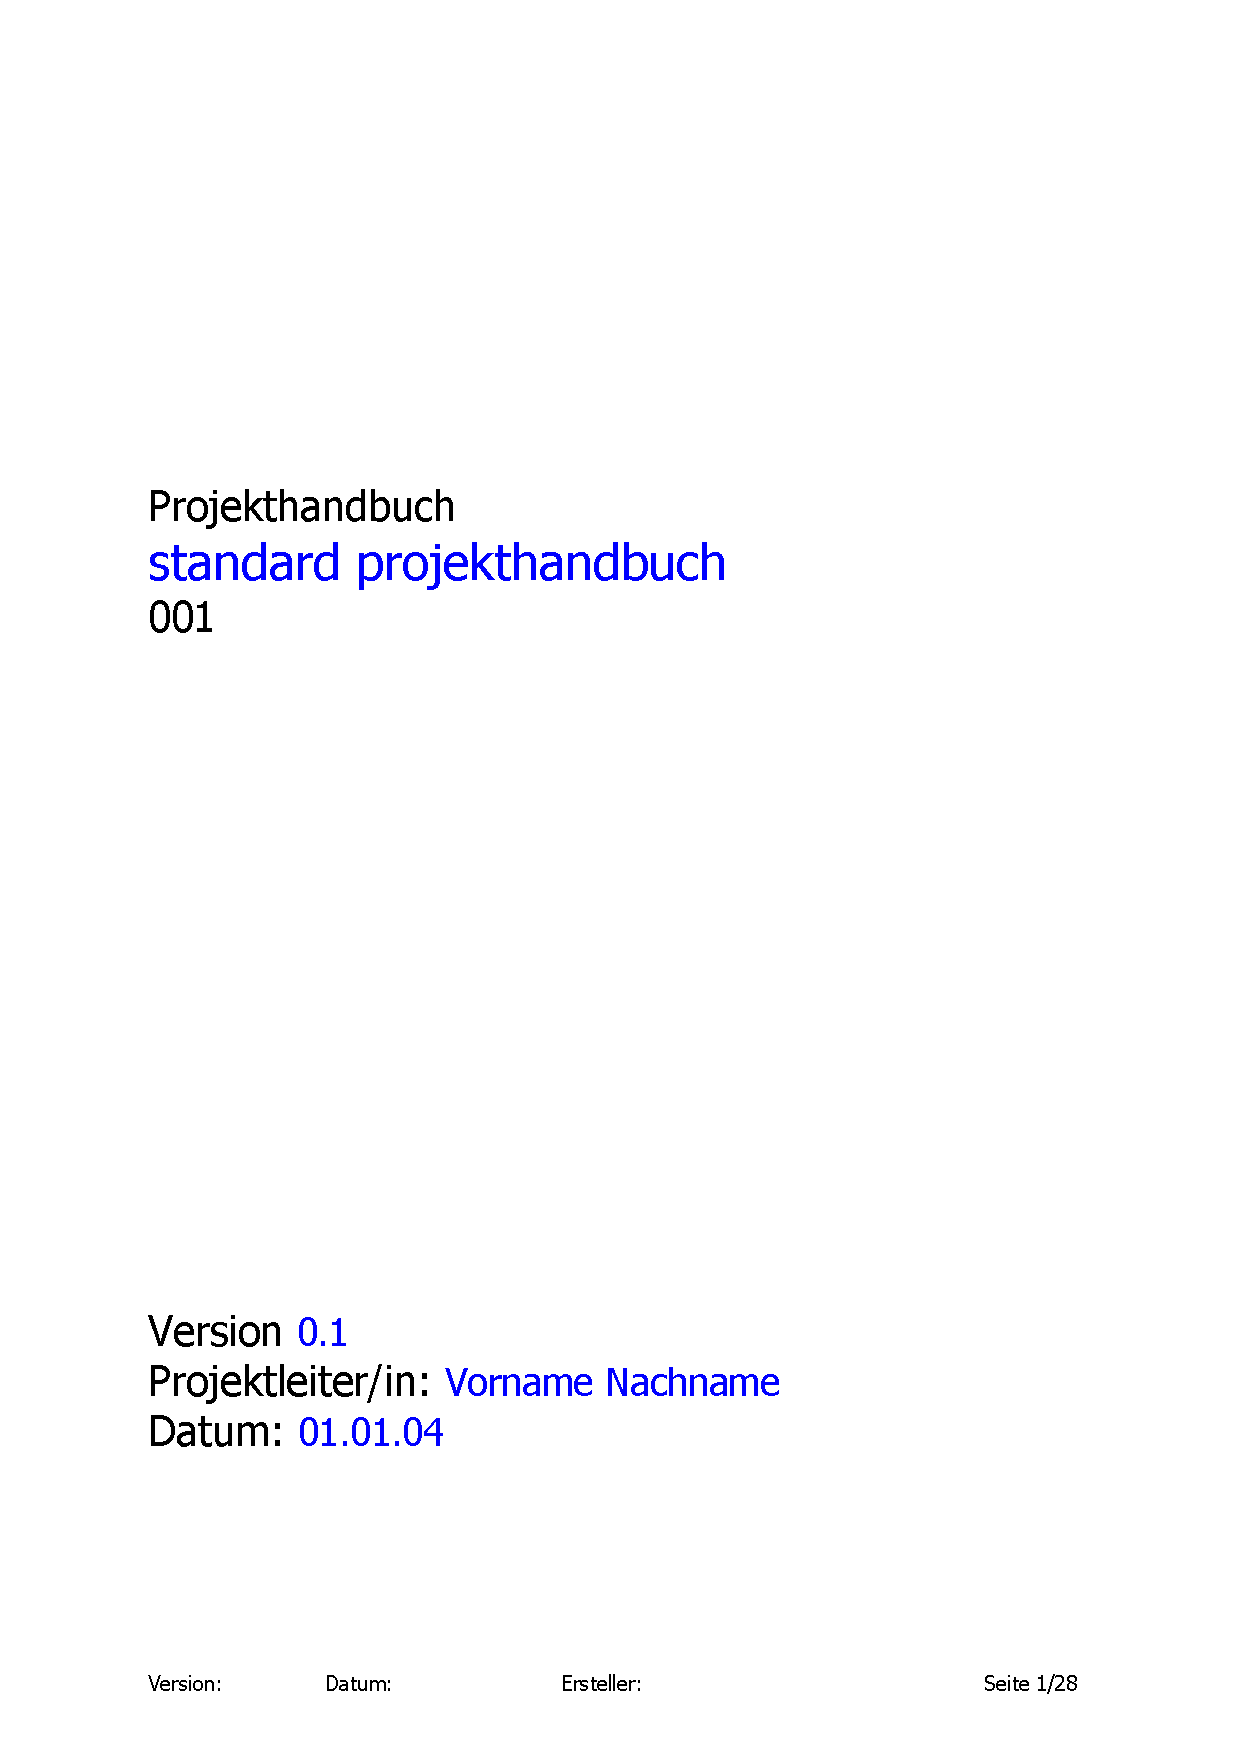
\includepdf[pages=1,scale=.9,pagecommand=\section{Projekthandbuch}]{doc/Projekthandbuch.pdf} % erste Seite des Projekthandbuchs mit Überschrift für Inhaltsverzeichnis
%\includepdf[pages=2-,scale=.9,pagecommand={}]{doc/Projekthandbuch.pdf} % einbinden des restlichen Projekthandbuchs

\section{Wochenberichte}
\subsection{Semih Can BURCAK}
\SecAuth{\emplLastA}


\subsubsection{KW38: 20.09.2021 bis 26.09.2021}
\begin{quote}
	\subsubsection*{Arbeit in der Schule}
	Nach der Besprechung mit Professor Rusch, haben wir über das Projekt diskutiert. Wir haben über den Antrag, Pflichtenheft, Verlauf des Projektes (wer was macht, wie man einzelne Meilensteine realisieren wird, welche Schnittstellen werden verwendet, welche Assets werden verwendet, was soll die Geschichte des Spiels sein etc.)
	
	\subsubsection*{Arbeit außerhalb der Schule}
	\begin{itemize}
		\item DA-Antrag, Pflichtenheft - ca 2h
		\item LaTeX und Virtual-Machine einrichten - 1h
		\item Unity Installation und Beginner Tutorials - 2h
	\end{itemize}
	Die Installation von LaTeX machte mir am Anfang Probleme aber ich habe es gelöst, indem ich den ganzen Prozess nochmals durchgemacht habe. DA-Antrag musste ich verbessern und manche Teile neu schreiben, hier habe noch zusätzlich die Sachen zum Spiel geschrieben und die anderen Teile des Projekt wurden von den entsprechenden Mitglieder geschrieben. Am Ende habe ich alles in einer Datei zusammengefasst. Bei dem Lastenheft/Pflichtenheft habe ich mein Teil bezüglich des Spiels und Projektmanagement geschrieben und anschließend es meinen Teamkollegen geschickt. Ich habe das Lastenheft am Sonntag geschickt, was meiner Meinung nach spät ist aber ich werde versuchen mehr diszipliniert zu arbeiten, damit ich meinen Teamkollegen kein Zeitdruck erzeuge.
	
	\subsubsection*{Was ist geplant für die Nächste Woche}
	Diese Woche werde ich mich auf Unity konzentrieren und viele Tutorials durchmachen. Da ich für ein nicht-existierendes Spiel keine Online-Funktion programmieren kann, werde ich schauen, dass wir das Spiel schnell wie möglichst für Online bereitmachen. Ich werde aber natürlich in dieser Zeit auch das Know-How für Onlinespielentwicklung erschaffen.
\end{quote}


\pagebreak
\subsubsection{KW 39: 27.09.2021 bis 03.10.2021}
\begin{quote}
	\subsubsection*{Arbeit in der Schule}
	Wir haben in der Schule Verbesserungsvorschläge bezüglich unseres Antrags vom Herrn Professor Rusch bekommen. Wir haben eine Stunde Zeit bekommen um den Antrag zu verbessern. Dies haben wir auch getan und anschließend im System des Bildungsministeriums abgegeben. Danach hat jeder Teammitglied seine eigenen Meilensteine definiert und es im Pflichtenheft geschrieben.  
	
	\subsubsection*{Arbeit außerhalb der Schule}
	\begin{itemize}
		\item DA-Antrag - 0.5h
		\item Unity Menu (UI) Tutorials - 2.5h\footcite{MenuTutorial}
	\end{itemize}
	Diese Woche habe ich angefangen Unity-UI zu üben. Dazu habe ich auf YouTube ein gutes Starter-Tutorial gefunden. Jedoch lief bei mir nicht alles wie geplant. Da ich Unity nicht so gut kenne, musste ich immer wieder mit Fehler kämpfen, z.B. die Buttons sind auf einmal nicht gegangen oder Unity erkennte mein Code bzw. die Funktionen im Code nicht mehr usw.. Ich konnte bisher diese Fehler nicht vollständig verbessern, denn sie erscheinen immer wieder und jedes Mal ist etwas anderes Falsch, also ich kann dieselbe Lösung, wie vorher, nicht anwenden. Herr Professor Rusch hat uns noch paar kleine Verbesserungsvorschläge gemacht bezüglich des Antrags, ich habe den Antrag verbessert und anschließend abgegeben.    
	
	\subsubsection*{Was ist geplant für die Nächste Woche}
	Ich werde nächste Woche schauen, dass ich ein Start-Menü erstelle und es meinen Teamkollegen zeige, damit wir uns auf ein Design einigen. Wenn ich mit dem Menü rasch fertig werde, werde ich über den Multiplayer-Modus (+Webserver) in Unity recherchieren. Ich werde auch schauen, dass wir jetzt von Typora auf LaTeX wechseln. 
\end{quote}

\pagebreak
\subsubsection{KW40: 04.10.2021 bis 10.10.2021}
\begin{quote}
	\subsubsection*{Arbeit in der Schule}
	Ich habe in der Schule weiter am Start-Menü geschaffen, ich war auf der Fehlersuche, wieso die Buttons nicht funktionieren. Ich habe dann festgestellt, dass ein EventHandler gefehlt hat, nachdem haben die Buttons funktioniert. Dann wurde die Funktion im Code von Unity nicht erkannt, ich habe die Lösung noch nicht gefunden. Wir haben auch über den Megacard-Kontroller gesprochen, welche Einzelteile wir brauchen, wie man den Akku wieder aufladen kann etc., bei Fragen haben wir uns an den Herrn Professor Zudrell-Koch gewendet. Nach der großen Pause (15:20) haben wir uns mit dem Herrn Professor Rusch in der Klasse getroffen und er hat uns gezeigt, wie man LaTeX und Gitlab verwendet, was sehr hilfreich war.
	
	\subsubsection*{Arbeit außerhalb der Schule}
	Ich habe meine Wochenberichte und Pflichtenheft auf LaTeX übertragen, am Anfang war es ein bisschen Kompliziert aber man kommt schnell im Rhythmus. Ich habe versucht Quellen einzufügen, aber es ist leider nicht gegangen, ich habe dann später entdeckt, dass ich Syntaxfehler hatte aber auch nach der Verbesserung wurde meine eingefügte Quelle im Quellenverzeichnis nicht gezeigt.
	
	Am Montag (11.10.2021) hat mir Herr Professor Rusch gezeigt wie man Quellen einfügt und somit habe ich das Problem lösen können.
	
	Ich habe das Start-Menü in Unity fertig gemacht. Ich musste mit vielen fehlern kämpfen, die Buttons haben auf einmal nicht funktioniert, ich musste ein EventSystem einfügen um das zu lösen. Dann hat Unity mein Code nicht erkannt, die Lösung dafür war: ich musste das GameObject selbst verwenden anstatt der C\#-Datei.
	
	Mehr konnte ich leider nicht machen, weil ich über das Wochenende krank geworden bin. 
	
	\begin{itemize}
		\item Wochenberichte und Pflichtenheft in LaTeX einfügen - 2h
		\item Start-Menü erstellen - 1.5h
	\end{itemize}

	\subsubsection*{Was ist geplant für die Nächste Woche}
	Ich werde schauen, dass ich die Menüs gut designe und über Multiplayerspielentwicklung in Unity (+Webserver) recherchiere.
\end{quote}
\pagebreak
\subsubsection{KW41: 11.10.2021 bis 17.10.2021}
\begin{quote}
	\subsubsection*{Arbeit in der Schule}
	Herr Professor Rusch hat uns gezeigt wie man Quellen einfügt in LaTeX. Danach habe ich gefunden, was mein Fehler war in Unity. Ich konnte die Buttons nicht drücken, ich habe dieses Problem gelöst, indem ich ein EventSystem eingefügt habe in meinem Projekt.
	
	\subsubsection*{Arbeit außerhalb der Schule}
	Ich war leider krank und konnte für die Diplomarbeit nichts machen.
	
	\subsubsection*{Was ist geplant für die Nächste Woche}
	siehe letzte Woche (KW40)
\end{quote}


\pagebreak
\subsubsection{KW42: 18.10.2021 bis 24.10.2021}
\begin{quote}
	\subsubsection*{Arbeit in der Schule}
	In der Schule habe ich über Online-Multiplayer-Spielentwicklung (OMSE) in Unity recherchiert. Es gibt eine große Auswahl von Services bzw. Bibliotheken, die man wählen kann für OMSE, aber ich habe Photon gewählt, weil Sie gratis einen cloudbasierten Webserver anbieten und das Service ist auf C\# basiert.
	
	Für Mehreres hatte ich leider keine Zeit mehr, da wir nach der zweiten Stunde für Maturafotos fort müssten.  
	
	\subsubsection*{Arbeit außerhalb der Schule}
	Ich habe ein Tutorial-Spiel\footcite{Karting Microgame Unity3D} heruntergeladen und habe angefangen mithilfe Photon, und mit einem entsprechenden Tutorial\footcite{Unity Photon Tutorial} dazu, das Spiel in ein Online-Multiplayer-Spiel zu umprogrammieren. Da es mein erstes Mal war mit Photon, musste ich zuerst mal die Lernkurve überwinden. Ich bin noch nicht fertig geworden mit dem Umprogrammieren. Ich habe geschafft das Spiel mit dem Server zu verbinden und Räume zu erstellen, ich konnte mit zwei Builds in den gleichen Raum beitreten.
	
	Ich habe mich diese Woche mit den Menü-Designs nicht beschäftigt, obwohl es geplant war. Weil, ich denke, dass es momentan nicht sehr nötig ist bzw. eine hohe Priorität hat.   
	
	\begin{itemize}
		\item Recherche über Photon - 1h
		\item Tutorial-Spiel auf Online-Spiel umprogrammiert - 3h
	\end{itemize}
	
	\subsubsection*{Was ist geplant für die Nächste Woche}
	Das Tutorial-Spiel fertig umprogrammieren.
\end{quote}
\pagebreak
\subsubsection{KW43: 25.10.2021 bis 31.10.2021}
\begin{quote}
	\subsubsection*{Arbeit in der Schule}
	**HERBSTFERIEN** 
	
	\subsubsection*{Arbeit außerhalb der Schule}
	Ich habe das Tutorial-Spiel\footcite{Karting Microgame Unity3D} entsprechend zu dem Tutorial\footcite{Unity Photon Tutorial} fertig umprogrammiert. Ich musste diese Woche nur noch die seperate Bewegung und Synchronisation der Spieler programmieren. Aber da der Code vom Spiel nicht von mir stammt und auch sehr kompliziert war, musste ich viel mit Fehlern kämpfen. Doch ein Fehler konnte ich nicht lösen. Der Bewegung-Code hatte noch die Photon-Bibliothek nicht und es erkannte sie auch nicht. Ich musste zuerst die Photon-Bibliothek Referenzen einfügen, was leider nicht nur mit einem Rechtsklick auf Referenzen zu machen war, obwohl es so machbar sein sollte, es hat mich sehr viel Zeit gekostet aber zumindest hat Visual Studio die Photon-Bibliothek erkennen können. Doch dann kam der nächste Fehler, der Code wurde nicht kompiliert von Unity. Ich habe den Fehler mit paar Tricks, wie z.B. sehr viele Leerzeichen einfügen, lösen können aber auch nachdem Unity mein Code kompiliert hat, bekam ich immer noch den Fehler, dass die Photon-Bibliothek nicht gebunden war und deshalb manche Sachen im Code nicht erkennt werden können.     
	
	\begin{itemize}
		\item Spiel fertig umprogrammiert - 1h
		\item Fehlersuche - 5h
	\end{itemize}
	
	\subsubsection*{Was ist geplant für die Nächste Woche}
	Eine Datenbank erstellen mit MySQL und es mit Unity verbinden.
\end{quote}
\pagebreak
\subsubsection{KW44: 01.11.2021 bis 07.11.2021}
\begin{quote}
	\subsubsection*{Arbeit in der Schule}
	**HERBSTFERIEN** 
	
	\subsubsection*{Arbeit außerhalb der Schule}
	Ich habe eine Datenbank erstellt mittels MySQL.
	Ich habe ein Login-Menü erstellt und einen einfachen Klick-Counter programmiert um Scores zu speichern können.
	Ich habe auch was sehr wichtiges gelernt, ich habe den Namen der Szene geändert bevor ich es gespeichert habe und alles hat sich gelöscht. Man muss die Szene immer speichern bevor man den Namen ändert.
	
	Ich habe auch Kapiteln "DIPLOMARBEIT DOKUMENTATION" und "DIPLOMA THESIS DOCUMENTATION" ergänzt.
	
	\begin{itemize}
		\item Fehlende Teile der Doku ergänzt - 1h
		\item Datenbank-Setup, Recherche über Unity und MySQL, Programmierung und Erstellung des Login-Menüs und Klick-Counter. -2.5h
	\end{itemize}
	
	\subsubsection*{Was ist geplant für die Nächste Woche}
	Die Datenbank mit Unity verbinden.
\end{quote}
\pagebreak

\subsubsection{KW45: 08.11.2021 bis 14.11.2021}
\begin{quote}
	\subsubsection*{Arbeit in der Schule}
	Wochenberichte verglichen und über die Doku diskutiert.
	Überschrifte und Sektionen der Doku und Wochenberichte diskutiert.	
	
	Wochenberichte von Manuel Rath exportiert auf LaTex.
	
	\subsubsection*{Arbeit außerhalb der Schule}
	Ich war leider mit der Schule beschäftigt und konnte für die DA nicht vieles machen.
	
	Menü Designs verschönert - 1h
	Musik eingefügt (Menüs) - 30min
	
	
	\subsubsection*{Was ist geplant für die Nächste Woche}
	Musik Überlappung Fehler beheben. Evlt. die Datenbank mit Unity verbinden.
	
	\subsubsection*{Welche Schwierigkeiten hat es gegeben}
	Die Musik überlappt sich bei jeder Rückkehr zum Start-Menü.
	
\end{quote}

\pagebreak

\subsubsection{KW46: 15.11.2021 bis 21.11.2021}
\begin{quote}
	\subsubsection*{Arbeit in der Schule}
	Fehlersuche Musik. Ich habe den Fehler nicht direkt lösen können und habe ein extra Menü erstellt das man nur am Anfang sieht und nicht wieder zurück kann und ich starte die Musik dort. 
	\subsubsection*{Arbeit außerhalb der Schule}
	Ich habe leider wegen Tests für die DA nichts machen können.
	
	\subsubsection*{Was ist geplant für die Nächste Woche}
	Die Datenbank mit Unity verbinden.
	
	\subsubsection*{Welche Schwierigkeiten hat es gegeben}
	-
	
\end{quote}

\pagebreak

\subsubsection{KW47: 22.11.2021 bis 28.11.2021}
\begin{quote}
	\subsubsection*{Arbeit in der Schule}
	Wir haben unsere Unity-Projekte mit Herrn Sönmez zusammengeführt. Ich habe die aktuelle Game-Scene mit der von Herr Sönmez gewechselt. 
	
	\subsubsection*{Arbeit außerhalb der Schule}
	Ich habe beim Tutorial weitergemacht und die Unity bzw. C\#-Teil und den PHP-Teil für die Datenbankverbindung programmiert. - 2h
		
	Fehlersuche Datenbankverbindung - 2h
	
	\subsubsection*{Was ist geplant für die Nächste Woche}
	Fehlerbehebung Datenbank
	
	\subsubsection*{Welche Schwierigkeiten hat es gegeben}
	Ich habe Syntaxfehler in meinen Codes gefunden und das Passwort für die Server-Connection (PHP) hatte ich falsch. URL für das PHP-Programm in C\# war auch nicht korrekt. Aber ich kann leider immer noch nicht auf das PHP-Programm zugreifen mit Unity.
	
\end{quote}

\pagebreak
\subsubsection{KW48: 29.11.2021 bis 05.12.2021}
\begin{quote}
	\subsubsection*{Arbeit in der Schule}
	Antrag für die Unityumgebung geschrieben und an den Herrn Rusch geschickt.
	Fehlersuche PHP und C\#, ich kann jetzt mit Unity auf das PHP-Programm zugreifen.
	Unity Package gekauft.
	
	\subsubsection*{Arbeit außerhalb der Schule}
	Fehlersuche Datenbank - 2h
	Recherche über andere Datenbanken - 1h
	
	\subsubsection*{Was ist geplant für die Nächste Woche}
	Datenbank Fehler beheben.
	
	\subsubsection*{Welche Schwierigkeiten hat es gegeben}
	Leider funktioniert die Verbindung noch nicht vollständig. Am Anfang konnte ich mit der Datenbank nicht verbinden, ich habe dann im Code WWW mit UnityWebRequest (weil WWW nicht mehr von Unity unterstütz wird) gewechselt und es hat funktioniert. Aber ich kann leider die Spieler nicht in die Datenbank einfügen.
	
\end{quote}

\pagebreak
\section{Wochenberichte}
\subsection{Semih SÖNMEZ}
\SecAuth{\emplLastB}



\subsubsection{KW38: 20.09.2021 bis 26.09.2021}
\begin{quote}

	\subsubsection*{Arbeit in der Schule}
	Besprechung Diplomarbeit mit Herrn Rusch: 1h
	
	Es wurde besprochen wie wir am Diplomarbeit arbeiten sollen. Jede Woche soll ein Wochenbericht geschrieben werden, welches am Schluss in die Dokumentation eingefügt wird. Das Wochenbericht entsteht aus den folgenden Punkten: 
	
	- Was wurde gemacht
	
	
	- Was ist geplant für die Nächste Woche
	
	
	- Welche Schwierigkeiten hat es gegeben
	
	
	- Schwierigkeiten oder Fragen die Aufgekommen sind
	
	- Jeder Schüler muss 150 Stunden außerhalb der Schule am Diplomarbeit arbeiten.
	
	
	Planung des Spiels. Wie soll das Spiel programmiert werden?
	
	Um das Spiel zu planen, soll ein Lastenheft und ein Pflichtenheft erstellt werden. Damit können wir unser Projektplanen und in kleine Arbeitspakete gliedern.
	
	\subsubsection*{Arbeit außerhalb der Schule}
	Virtuelle Machine: Latex heruntergeladen und installiert 1h
	
	Antrag auf die Diplomarbeit fertig geschrieben 1h
	
	Lastenheft erstellt 1h
	
	Unity-tutorial abgeschlossen 2h
	
	\subsubsection*{Was ist geplant für die Nächste Woche?} 
	Es soll mit der Programmierung des Spiels angefangen werden.
	
	Der Charakter des Spiels wird zuerst entwickelt 
	
	\subsubsection*{Welche Schwierigkeiten hat es gegeben} 
	Es war schwer, das Spiel aufzuteilen. Wer macht was ?
\end{quote}

\pagebreak


\subsubsection{KW39: 27.09.2021 bis 03.10.2021}
\begin{quote}
	\subsubsection*{Arbeit in der Schule}
	  Besprechung Diplomarbeit mit Herrn Rusch \textbf{1h}
	  
	  Die Arbeit wurde gerecht aufgeteilt, so dass alle Mitglieder gleich
	  viel Arbeit haben. Wer macht was? \textbf{1h}
	  
	  Planung des Spiels. Wie soll das Spiel programmiert werden?
	  \textbf{1h}
	  
	  Virtuelle Machine: Latex heruntergeladen und installiert \textbf{1h}
	  
	
	\subsubsection*{Arbeit außerhalb der Schule}
	  Antrag auf die Diplomarbeit fertig geschrieben \textbf{1h}
	  
	  Lastenheft erstellt \textbf{1h}
	  
	  Unity-tutorial abgeschlossen \textbf{2h}
	
	\subsubsection*{Was ist geplant für die Nächste Woche?} 
	
	  Es soll mit der Programmierung des Spiels angefangen werden
	
	    Der Charakter des Spiels wird als zuerst entwickelt
	
	\subsubsection*{Welche Schwierigkeiten hat es gegeben?} 
	
	  Es war schwer, das Spiel aufzuteilen.
\end{quote}

\pagebreak


\subsubsection{KW40: 04.10.2021 bis 10.10.2021}
\begin{quote}
	\subsubsection*{Arbeit in der Schule}
	
	
	Besprechung mit Herrn Rusch:
	
	Wir haben gemeinsam mit Herrn Rusch das Programm Latex auf unserer
	Virtual Machine installiert. Anschließend haben wir unser Repository, die wir im Gitlab erstellt haben, in unserem PC geklont.
	
	Dies wurde mit dem folgenden Befehl realisiert: git clone {[}url-vom
	Projekt{]}.
	
	\subparagraph{\texorpdfstring{Daten uplod:
	}{Daten uplod: }}
	
	Um Daten auf GitLab hochzuladen, werden folgende Befehle ausgeführt:
	
	Zuerst muss im Terminal auf unser Repository-Ordner navigiert werden:
	
	\texttt{ls\ -l} : Inhalt des Verzeichnis
	
	\texttt{cd\ Verzeichnisname} : in den Ordner wechseln
	
	\texttt{git\ status} : Abfrage ob im lokalen Repository etwas verändert
	wurde
	
	\texttt{git\ add}. : eine Änderung aus dem Arbeitsverzeichnis wir zur
	Staging-Umgebung hinzugefügt
	
	\texttt{git\ commit\ -am\ "name"} : Der Befehl committet den Snapshot im
	Staging-Bereich in die Projekt-Historie
	
	\texttt{git\ push} : Änderung werden hochgeladen
	
	\subparagraph{Daten download:}
	
	hier muss wieder auf unseren Repository-Ordner navigiert werden.
	
	\texttt{git\ pull} : Inhalte vom Repository herunterladen um das lokale
	Repository zu aktualisieren
	
	Danach hat uns Herr Rusch eine Einführung zum Programm LaTex gegeben.
	
	
	\paragraph{Arbeit außerhalb der Schule}
	
	
	Ich habe am Programm, welches für die Bewegung vom Charakter dient,
	weitergearbeitet.
	
	Es wurde ein Animator Controller erstellt, bei der 2 Zustände im State
	Machine definiert worden sind. Nachdem das Spiel gestartet wird(Entry),
	wird sofort der Zustand idle übernommen. Mit der Animation idle steht
	der Charakter ohne Bewegung. Doch wenn die Boolvariable IsWalking wahr
	wird, geht der Zustand von idle zu run, welches den Charakter in
	Bewegung setzt. Wenn die Boolvariable IsWalking wieder unwahr wird,
	kährt sie zum default state, also zum idle wieder zurück. Die
	Animationen wurden vom Character Pack: Free Sample entnommen.
	\begin{center}
		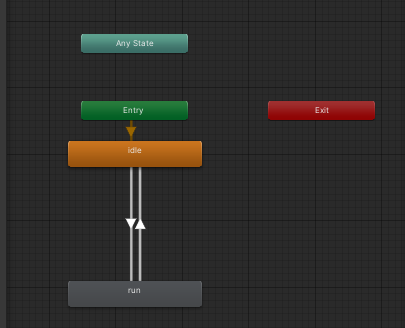
\includegraphics[frame, height=6cm]{img/SemihSoenmez_IMG/StateMachine_SS_KW41_041021.png}
	\end{center}

	Anschließend wurde der Animator Controller zum Prefab Model zugewiesen.
	
	
	\subsubsection*{Was ist geplant für die Nächste Woche}
	Es soll mit dem Character Controller Programm weitergearbeitet werden.
\end{quote}	


\pagebreak


\subsubsection{KW41: 11.10.2021 bis 17.10.2021}

\begin{quote}
	\subsubsection*{Arbeit in der Schule}
	
	Besprechung mit Herrn Rusch:
	
	Wir haben Git auf unserem Windows Rechner installiert. Anschließend
	wurde eine neue SSH generiert und ins Gitlab eingefügt. Danach wurde das
	Projekt geklont und die Unity-Projekte hochgeladen. Somit haben wir
	jetzt sowohl im Windows-Rechner als auch in der Virtual Machine Zugriff
	auf das Git, wo die Arbeit immer gespeichert werden kann.
	
	
	\subsubsection*{Arbeit außerhalb der
	Schule}
	
	Da ich im Git ständig zur Diplomarbeitsordner navigieren musste und dies
	sehr Zeit in Anspruch nahm, habe ich eine Lösung gefunden. Im
	Git-Ordner C:\textbackslash Program
	Files\textbackslash Git\textbackslash etc gibt es ein File namens
	bash.bashrc, welches beim Starten des Gits aufgerufen wird. In dieser
	Datei habe ich folgendes eingefügt:
	
	\texttt{\#set\ Diplomarbeit\ directory\ as\ default\ directory
	cd\ C:/HTL\_2021-22/Diplomarbeit/mazerun}
	
	Anschließend habe am Programm, welches für die Bewegung vom Charakter
	dient, weitergearbeitet und versucht die Bugs zu lösen.
	
	
	\subsubsection*{Was ist geplant für die Nächste
	Woche}
	
	Das Programm für die CharacterController soll fertig programmiert
	werden.
\end{quote}

\pagebreak



\subsubsection{KW42 + KW43:}
\begin{quote}
	\subsubsection*{Arbeit in der Schule}
	
	Im Unity Asset Store wurde der Character Pack: Free Sample
	heruntergeladen und in das Projekt eingefügt. Anschließend wurde der
	Prefab Model in die Scene eingefügt. In der Scene wurde auch mit einem
	3D-Cube der Boden erstellt. Danach wurde der Animator
	Controller und das Character Movement Programm, dem Charakter
	zugewiesen.
	
	Ergebnis: Der Charakter kann grundlegende Bewegungen wie Renen, Drehen
	und Springen ohne Probleme ausführen.
	\begin{figure}
		\centering
		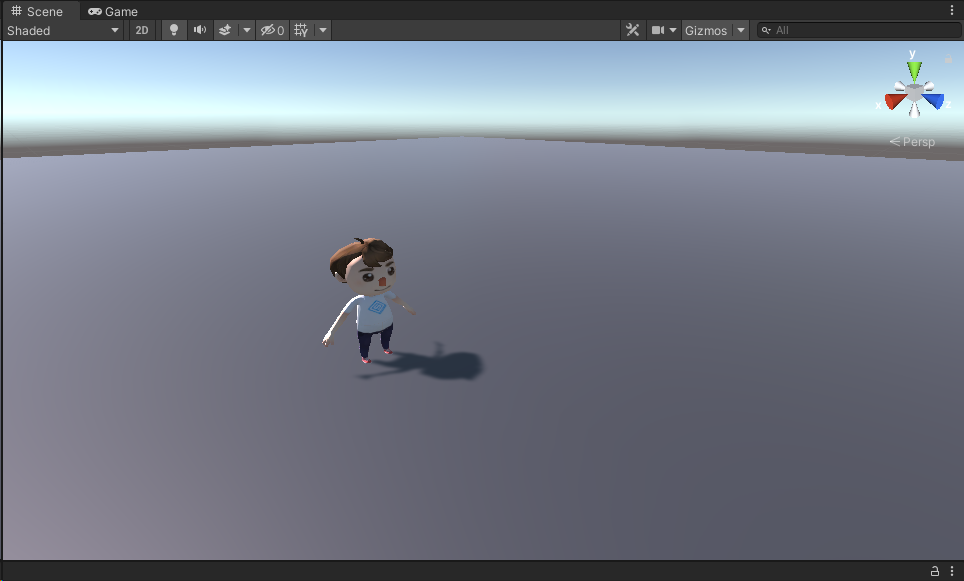
\includegraphics[width=0.6\linewidth]{img/SemihSoenmez_IMG/Main-Charakter_SS_KW45_131121}
		\caption{}
		\label{fig:main-charaktersskw45131121}
	\end{figure}
	
	
	Anschließend habe ich ein bisschen rechechiert wie ich die Gegner
	programmieren soll, da dies meine nächste Aufgabe ist.

	\subsubsection*{Arbeit außerhalb der Schule}
	Meine nächste Aufgabe ist es die Gegner zu programmieren. Dafür habe ich
	auf der Seite \url{www.mixamo.com} ein Lehrer-Charakter und eine
	Lauf-Animation heruntergeladen und sie im Projekt eingefügt.
	
	Links:


	Youtube-tutorial für Charakter: \footcite{CharakterTutorial}
	
	Walking Animation: \footcite{WalkingAnimation}
	
	Charakter Leonard: \footcite{LehrerCharakter}
	
	Der eingefügte Charakter war in der Scene grau zu sehen. Also habe ich
	sein Material vom Charakter im Inspector window extrahiert. Anschließend
	war der Charakter wieder bunt zu sehen.

	\begin{figure}
		\centering
		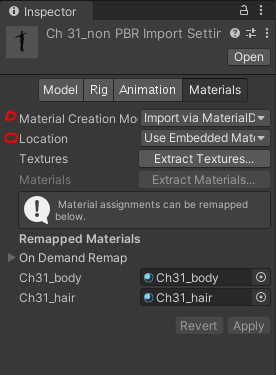
\includegraphics[width=0.3\linewidth]{../../mazerun/dokumentation/img/SemihSoenmez_IMG/Inspector_SS_KW44_251021}
		\caption{}
		\label{fig:inspectorsskw44251021}
	\end{figure}

	
	Jetzt muss dem Charakter die Walkinganimation zugewiesen werden.
	
	Inspector window: Rig:
	
	\begin{itemize}
		\item
		Animation Type auf "Humanoid"" und Avatar Definiton auf "Copy from
		other Avatar" umgestellt
		\item
		Beim Source den teacher Avatar ausgewählt
	\end{itemize}
	
	Danach wurde ein Animator Controller erstellt, in der wir unsere
	Animation eingefügt haben. Wie im Bild zusehen ist, wird beim Starten
	des Spiels, der Start Walking Animation durchgeführt.
	\begin{center}
		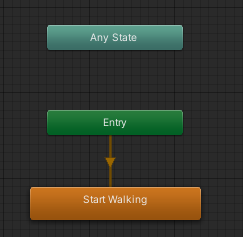
\includegraphics[frame, height=6cm]{img/SemihSoenmez_IMG/StateMachine_SS_KW44_251021.png}
	\end{center}
\end{quote}


\pagebreak

\subsubsection{KW44: 01.11.2021 bis 08.11.2021}
\begin{quote}
	\subsubsection*{Arbeit in der Schule}
	Die Funktion vom Lehrer Charakter: Wenn unser Hauptcharakter(Schüler) sich im Blickwinkel vom Lehrer befindet soll das Spiel beendet(Game Over) werden.
	
	 Ich habe schon diese Funktion im Projekt John Lemon beim Charakter Gargoyle verwendet. Also wurde aus dem Projekt John Lemon, der Charakter Gargoyle herauskopiert und in unser Projekt eingefügt. Anschließend wurde der Gargoyle Charakter getestet. Leider hat es nicht funktioniert.
	 
	 \subsubsection*{Arbeit außerhalb der Schule}
	Ich habe versucht das Problem zu beheben.
	
	\subsubsection*{Welche Schwierigkeiten hat es gegeben}
	Der Charakter Gargoyle hat nicht funktioniert, obwohl es im anderen Projekt funktioniert hat.
\end{quote}


\pagebreak

\subsubsection{KW45: 08.11.2021 bis 14.11.2021}
\begin{quote}
	\subsubsection*{Arbeit in der Schule}
	Da der Gargoyle Charakter nicht funktioniert hat habe ich die Schritte nochmals wiederholt.
	- import vom JL-Game folgendes: JohnLemon, Gargoyle, FaderCanvas
	
	- export in das eigene Spiel
	
	- Prefab Modelle von JohnLemon und Gargoyle in die Scene eingefügt
	
	- FaderCanvas prefab eingefügt welches folgende Bilder beinhaltet:
		-ExitlmageBackground
		-CaughtlmageBackground
		
	  Der CaughtImage wird angezeigt wenn der Gargoyle Charakter den Haupcharakter in seiner PointOfView hat.
	  
	- Das PrefabModell GameEnding wurde auch vom JL-Game importiert.
	  Funktion von GameEnding: wenn der Character den Ziel(GameEnding Cube) erreicht, wird ExitlmageBackground angezeigt.
	  
	- Ergebnis: Wenn J.L im Blickwinkel vom Gargoyle ist wird Caughtlmage angezeigt und wenn J.L das Ziel erreicht wird Exitlmage angezeigt.
	
	- Das GameEnding Programm wurde im J.L Kurs in den Sommerferien geschrieben.
	
	 Abbildung \ref{fig:gameviewsskw45131122}
	  \begin{figure}
	  	\centering
	  	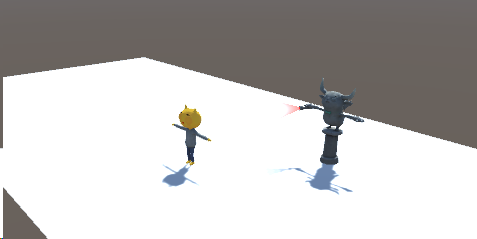
\includegraphics[width=0.5\linewidth]{img/SemihSoenmez_IMG/GameView_SS_KW45_131122}
	  	\caption{}
	  	\label{fig:gameviewsskw45131122}
	  \end{figure}
	\subsubsection*{Arbeit außerhalb der Schule}
	-Das Programm soll jetzt auch für unsere Charaktere funktionieren.
	
	 Unsere Charaktere: Hauptcharakter Schüler: Abbildung\ref{fig:main-charaktersskw45131121}
	 
	 Lehrer Charakter: Abbildung \ref{fig:lehrercharakterss151121}
	 \begin{figure}
	 \centering
	 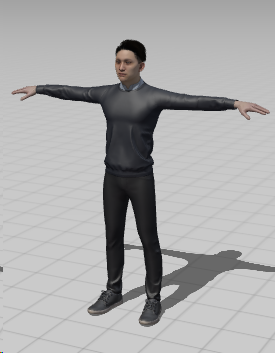
\includegraphics[width=0.3\linewidth]{img/SemihSoenmez_IMG/LehrerCharakter_SS_151121}
	 \caption{}
	 \label{fig:lehrercharakterss151121}
	 \end{figure}
	 					
	 					
	- Hauptcharakter Schüler wurde in die Scene eingefügt und die Parameter von Gargoyle für den Hauptcharakter angepasst.
	
	Ergebnis: Gargoyle erkennt den Hauptcharakter.
	
	- Charakter Lehrer wurde in die Scene eingefügt.
	
	
	
	\subsubsection*{Was ist geplant für die Nächste Woche}
	Die Funktion vom Charakter Gargoyle soll dem Charakter Lehrer implementiert werden.
	Ein dynamischer Gegner soll entwickelt werden, wie z.B. der Charakter Ghost.
	
	\subsubsection*{Welche Schwierigkeiten hat es gegeben}
	Die Funktionen von Charakteren richtig Laufen zu bringen.
	
\end{quote}

\pagebreak

\subsubsection{KW46: 15.11.2021 bis 21.11.2021}
\begin{quote}
	\subsubsection*{Arbeit in der Schule}
	Der Ghost Charakter wurde eingefügt, welche ein dynamischer Gegner ist. Der Ghost bewegt sich in einer bestimmten Umgebung und schaut ob er den Charakter in seiner Point of View hat. 
	\subsubsection*{Arbeit außerhalb der Schule}
	Ich konnte in GIT meine Arbeit nicht speichern, da ein Fehler auftauchte.
	Ich habe im Internet recherchiert und in einem Beitrag gelesen, dass man auf Git nicht mehr als 2GB Daten hochladen soll, da sonst Probleme auftauchen könnten. Doch unsere Repository war ca. 4Gb groß. Nachdem wir die unwichtigen Dateien gelöscht haben und ich die Repository nochmals geclont habe, hat alles wieder funktioniert. 
	\subsubsection*{Was ist geplant für die Nächste Woche}

	\subsubsection*{Welche Schwierigkeiten hat es gegeben}
	
	\subsubsection*{Notizen für mich selber}
\end{quote}

\pagebreak


\subsubsection{KW47: 01.11.2021 bis 08.11.2021}
\begin{quote}
	\subsubsection*{Arbeit in der Schule}
		Die Scenen von meinem Partner habe ich in den Ordner, wo meine Scenen sind hineinkopiert um sie nacher zu verbinden.
	\begin{figure}
		\centering
		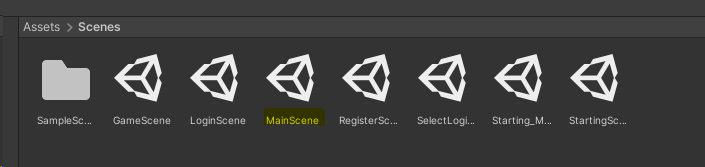
\includegraphics[width=0.7\linewidth]{img/SemihSoenmez_IMG/KW47_unity_scenes2}
		\caption{}
		\label{fig:kw47unityscenes2}
	\end{figure}
		Semih Can hat folgende Funktion programmiert: Wenn im Menü auf spielen gedrückt wird, wird der Main-Scene, wo unser Spiel ist gestartet. 
	
	\subsubsection*{Arbeit außerhalb der Schule}
	Kamera mit der Cinemachine-Funktion von Unity programmieren. Das Cinemachine Brain verwaltet alle virtuellen Kameras und entscheidet, welcher virtuelle Kamera die eigentliche Kamera folgen soll.
	
	\subsubsection*{Welche Schwierigkeiten hat es gegeben}

\end{quote}


\pagebreak

\pagebreak

\end{document}
